\documentclass[a4paper,12pt]{article}
\usepackage[utf8]{inputenc}
\usepackage[T2A]{fontenc}
\usepackage[russian,english]{babel}
\usepackage{graphicx}
\usepackage{amsmath, amssymb, amsthm}
\usepackage{algorithm}
\usepackage{algpseudocode}
\usepackage{geometry}
\usepackage{enumitem}
\usepackage{hyperref}
\usepackage{mathtools}
\usepackage{subcaption}
\usepackage{wrapfig}
\usepackage{float}
\usepackage{tikz}
\usetikzlibrary{arrows.meta, shapes, positioning, shadows, fit, decorations.markings}
\geometry{left=20mm, right=20mm, top=20mm, bottom=20mm}

\newtheorem{theorem}{Теорема}
\newtheorem{lemma}{Лемма}
\newtheorem{definition}{Определение}
\newtheorem{proposition}{Утверждение}

\title{Локальные свойства нейронных сетей через призму гессианов слоёв}
\author{Максим Большим}
\date{\today}

\begin{document}

\maketitle

\begin{abstract}
  В данной работе представлен новый подход к анализу нейронных сетей, основанный на исследовании локальных
  свойств их параметрического пространства с помощью матриц Гессе. Введено понятие локального гессиана,
  позволяющее анализировать геометрию функционального пространства отдельных слоев нейронной сети. Предложены
  методы количественной оценки таких феноменов, как переобучение и недостаточная аппроксимирующая способность
  моделей, через спектральные характеристики локальных гессианов. Проведённый анализ 111 экспериментов на 37
  датасетах выявил закономерности в структуре локальных матриц гессиана на различных этапах обучения,
  что может служить основой для дальнейшего анализа и совершенствования архитектур нейронных сетей.
\end{abstract}

\section{Введение}

Глубокие нейронные сети продемонстрировали выдающиеся результаты во многих областях, включая компьютерное
зрение, обработку естественного языка и прочие задачи машинного обучения \cite{lecun2015deep,
goodfellow2016deep}. Однако, несмотря на их практический успех, остаётся открытым вопрос о том, почему одни
архитектуры превосходят другие и как формально и систематизированно улучшать дизайн нейронных сетей.
Эмпирический подход, основанный на методе проб и ошибок, становится всё более затратным с ростом размеров
моделей и объёмов данных.

Ряд работ показывает, что анализ кривизны ландшафта функции потерь через гессианы и родственные спектральные
инструменты может пролить свет на динамику обучения и обобщающую способность моделей
\cite{sagun2017empirical, maheswaranathan2019universality, lee2019wide, arora2019finegrained}. В настоящем
исследовании выдвигается тезис о том, что локальные свойства параметрического пространства нейронной сети
могут дать предварительную оценку внутренних свойств модели уже на ранних этапах обучения
\cite{poole2016transient}. Конкретно, мы предлагаем использовать локальные матрицы Гессе — матрицы вторых
производных целевой функции по параметрам отдельных слоёв — для анализа геометрии пространства параметров.

Концепция локального гессиана позволяет формализовать и количественно измерить геометрические свойства
пространства параметров в окрестности точки оптимизации. В частности, мы показываем, что спектр
локального гессиана, такой как распределение собственных значений и их структура
\cite{ghorbani2019investigation}, тесно связан с функциональными свойствами соответствующих слоёв нейронной сети.

Основные вклады настоящей работы:
\begin{itemize}
  \item Введение математически строгого определения локального гессиана для функциональных блоков нейронной сети
  \item Детальный анализ спектральных свойств локальных гессианов в процессе обучения нейронных сетей
  \item Исследование геометрической интерпретации пространства параметров нейронной сети через призму
    локальных гессианов
\end{itemize}

Полученные результаты не только углубляют наше теоретическое понимание глубоких нейронных сетей, но и
открывают новые перспективы для изучения их внутренней динамики.

\section{Математический аппарат нейронных сетей}

\subsection{Определение и структура нейронной сети}

\begin{definition}
  Нейронная сеть $\mathcal{F}: \mathbb{R}^d \rightarrow \mathbb{R}^m$ представляет собой параметризованную
  функцию с параметрами $\theta \in \mathbb{R}^P$, отображающую входные данные $x \in \mathbb{R}^d$ в
  выходное пространство через последовательность функциональных преобразований. Обозначим через
  $\mathcal{F}(x; \theta)$ результат применения сети к входным данным при заданных параметрах $\theta$.
\end{definition}

\begin{definition}
  Функциональным блоком (слоем) $C_i$ нейронной сети $\mathcal{F}$ называется пара модулей $(P_i, A_i)$, где:
  \begin{itemize}
    \item $P_i: \mathbb{R}^{d_i} \times \mathbb{R}^{p_i} \rightarrow \mathbb{R}^{q_i}$ -- параметризованное
      преобразование с параметрами $\theta_i \in \mathbb{R}^{p_i}$.
    \item $A_i: \mathbb{R}^{q_i} \rightarrow \mathbb{R}^{q_i}$ -- функция активации (потенциально тождественная)
  \end{itemize}
\end{definition}

\begin{definition}
  Нейронную сеть $\mathcal{F}$ можно представить как композицию $n$ функциональных блоков:
  \begin{equation}
    \mathcal{F}(x; \theta) = (C_n \circ C_{n-1} \circ \ldots \circ C_1)(x),
  \end{equation}
  где $C_i(z) = A_i(P_i(z; \theta_i))$ для входа $z$ и $\theta = \{\theta_1, \theta_2, \ldots, \theta_n\}$ --
  полный набор параметров сети.
\end{definition}

Такое представление нейронной сети позволяет провести анализ каждого функционального блока отдельно, что важно
для локального анализа свойств сети. Декомпозиция сложной модели на более простые составляющие является
ключевым методологическим приемом, который позволяет применить инструменты спектрального анализа к отдельным
компонентам.

\subsection{Промежуточные представления и функции активации}

\begin{definition}
  Промежуточным представлением $z_i$ называется вход в блок $C_i$:
  \begin{equation}
    z_i =
    \begin{cases}
      x, & \text{если } i = 1 \\
      (C_{i-1} \circ \ldots \circ C_1)(x), & \text{если } i > 1
    \end{cases}
  \end{equation}

  Соответственно, выход блока $C_i$ обозначается как:
  \begin{equation}
    y_i = C_i(z_i) = A_i(P_i(z_i; \theta_i))
  \end{equation}
\end{definition}

Промежуточные представления играют важную роль в анализе нейронных сетей, поскольку они содержат информацию о
том, как входной сигнал преобразуется на каждом этапе обработки. Особый интерес представляет исследование
геометрии этих промежуточных представлений и их взаимосвязь с параметрами соответствующих слоев.

\begin{definition}
  Для блока $C_i$ определим локальную скалярную функцию $S_i: \mathbb{R}^{p_i} \rightarrow \mathbb{R}$ как:
  \begin{equation}
    S_i(\theta_i) = \varphi(A_i(P_i(z_i; \theta_i))),
  \end{equation}
  где $\varphi: \mathbb{R}^{q_i} \rightarrow \mathbb{R}$ -- функция агрегации, обычно $\varphi(y) =
  \sum_{j=1}^{q_i} y_j$.
\end{definition}

Скалярная функция представляет собой способ оценки влияния параметров конкретного слоя на его выход
при фиксированном входе. Эта функция будет ключевой для определения локального гессиана в следующем разделе.

\subsection{Типичные реализации в нейросетях}

В контексте современных нейронных сетей часто используются следующие реализации компонентов:
\begin{itemize}
  \item $P_i$ -- линейное преобразование $P_i(z_i; \theta_i) = W_i z_i + b_i$, где $\theta_i = \{W_i, b_i\}$
  \item $A_i$ -- нелинейная функция активации, например, ReLU, Sigmoid или Tanh
  \item $\varphi(y_i) = \sum_{j=1}^{q_i} y_{i,j}$ -- суммирование всех компонент выходного вектора
\end{itemize}

Эти определения и обозначения будут использоваться во всех последующих разделах данной работы для обеспечения
математической строгости и последовательности.

\section{Локальные гессианы нейронной сети}

\subsection{Определение локального гессиана}

\begin{definition}
  Локальной матрицей Гессе $H_i \in \mathbb{R}^{p_i \times p_i}$ (далее для краткости — локальный гессиан,
  $LH_i$) для блока $C_i$ называется матрица вторых
  производных скалярной функции $S_i$ по параметрам $\theta_i$:
  \begin{equation}
    H_i = \nabla_{\theta_i}^2 S_i(\theta_i) = \left[ \frac{\partial^2 S_i(\theta_i)}{\partial \theta_{i,j}
    \partial \theta_{i,k}} \right]_{j,k=1}^{p_i}
  \end{equation}
\end{definition}

Анализ этой матрицы позволяет получить информацию о:

\begin{itemize}
  \item Степени нелинейности преобразования, выполняемого слоем
  \item Взаимосвязи между параметрами и их влиянии на выход слоя
  \item Геометрических свойствах пространства параметров
  \item Чувствительности слоя к малым изменениям параметров
\end{itemize}

В дифференциальной геометрии гессиан функции в точке определяет квадратичную форму, которая аппроксимирует
кривизну поверхности уровня этой функции. В контексте нейронных сетей $LH_i$ характеризует кривизну
функционального отклика слоя в пространстве его параметров \cite{dangel2019modular}. При анализе поверхности
следует учитывать знак собственных значений $LH_i$ и их распределение, так как это определяет
локальную геометрию.

\subsection{Эффективное вычисление $LH_i$}

Анализ нейронных сетей с использованием $LH_i$ представляет собой эффективный инструмент, однако из-за
квадратичной зависимости размера данной матрицы от числа параметров её прямое применение часто оказывается
вычислительно непрактичным. В связи с этим на практике широко применяются различные методы аппроксимации
$LH_i$ \cite{carlon2024, hare2024, martens2010, nocedal1980}. В данном разделе предлагается методика работы
с $LH_i$, позволяющая обойти указанные ограничения.

Для эффективного вычисления $LH_i$ предлагается алгоритм, основанный на последовательном
вычислении строк матрицы.

\begin{lemma}
  Элементы матрицы Гессе $H_i$ можно вычислять последовательно по строкам:
  \begin{equation}
    \begin{aligned}
      g_i &= \nabla_{\theta_i} S_i(\theta_i) = \left[ \frac{\partial S_i}{\partial \theta_{i,j}} \right]_{j=1}^{p_i} \\
      H_i[j,:] &= \nabla_{\theta_i} g_{i,j} = \nabla_{\theta_i} \left( \frac{\partial S_i}{\partial
      \theta_{i,j}} \right)
    \end{aligned}
  \end{equation}
\end{lemma}

\begin{proof}
  По определению матрицы Гессе, её элемент $H_i[j,k]$ равен:
  \begin{equation}
    H_i[j,k] = \frac{\partial^2 S_i(\theta_i)}{\partial \theta_{i,j} \partial \theta_{i,k}}
  \end{equation}

  Если обозначить $g_{i,j} = \frac{\partial S_i}{\partial \theta_{i,j}}$, то
  \begin{equation}
    H_i[j,k] = \frac{\partial g_{i,j}}{\partial \theta_{i,k}}
  \end{equation}

  Таким образом, $j$-я строка $H_i$ представляет собой градиент $j$-й компоненты градиента функции $S_i$.
\end{proof}

Это позволяет значительно сократить вычислительные затраты при работе с большими моделями, так как не требует
одновременного хранения в памяти всей матрицы Гессе размером $p_i \times p_i$.

Предложенный метод особенно важен при анализе современных глубоких нейронных сетей, содержащих миллионы
параметров, поскольку полная матрица $LH_i$ для таких моделей была бы непомерно большой.
Локальный подход не
только делает вычисления практически реализуемыми, но и позволяет сосредоточиться на анализе отдельных
компонентов сети, что часто более информативно, чем глобальный анализ.

\subsection{Алгоритм вычисления локального гессиана}

\begin{algorithm}
  \caption{Вычисление локальных гессианов нейронной сети}
  \begin{algorithmic}[1]
    \Require Нейронная сеть $\mathcal{F}$, входные данные $x \in \mathbb{R}^d$, функция агрегации $\varphi$
    \Ensure Набор локальных матриц Гессе $\{LH_1, LH_2, \ldots, LH_n\}$

    \State Разбить $\mathcal{F}$ на функциональные блоки $\{C_1, C_2, \ldots, C_n\}$, где $C_i = (P_i, A_i)$

    \For{$i = 1$ до $n$}
    \State Вычислить $z_i = (C_{i-1} \circ \ldots \circ C_1)(x)$ \Comment{Вход в блок $C_i$}
    \State Вычислить $y_i = A_i(P_i(z_i; \theta_i))$ \Comment{Выход блока $C_i$}
    \State Вычислить $S_i = \varphi(y_i)$ \Comment{Скалярная функция блока}

    \State Вычислить градиент $g_i = \nabla_{\theta_i} S_i$

    \State Инициализировать $LH_i \in \mathbb{R}^{p_i \times p_i}$ нулевой матрицей

    \For{$j = 1$ до $p_i$}
    \If{$g_{i,j}$ не является константой относительно $\theta_i$}
    \State Вычислить $LH_i[j,:] = \nabla_{\theta_i} g_{i,j}$
    \Else
    \State $LH_i[j,:] = \vec{0}$
    \EndIf
    \EndFor
    \EndFor

    \State \Return $\{LH_1, LH_2, \ldots, LH_n\}$
  \end{algorithmic}
\end{algorithm}

\subsection{Математические детали реализации}

\subsubsection{Вычисление градиента $g_i$}
В контексте автоматического дифференцирования градиент $g_i$ вычисляется как:
\begin{equation}
  g_i = \nabla_{\theta_i} S_i = \frac{\partial S_i}{\partial y_i} \cdot \frac{\partial y_i}{\partial P_i}
  \cdot \frac{\partial P_i}{\partial \theta_i}
\end{equation}

где:
\begin{itemize}
  \item $\frac{\partial S_i}{\partial y_i} = \nabla_{y_i} \varphi(y_i)$ -- градиент функции агрегации
  \item $\frac{\partial y_i}{\partial P_i} = \nabla_{P_i} A_i(P_i)$ -- якобиан активационной функции
  \item $\frac{\partial P_i}{\partial \theta_i}$ -- якобиан параметризованного преобразования по его параметрам
\end{itemize}

\begin{figure}[ht]
  \centering
  \begin{tikzpicture}[
      box/.style={draw, minimum width=1.2cm, minimum height=3cm, thick},
      smallbox/.style={draw, minimum width=1cm, minimum height=3cm, thick},
      arrow/.style={-Stealth, line width=1pt},
    ]
    % 1) Стрелка над всеми слоями
    \draw[arrow] (-2,4) -- (10,4);
    \node[draw, fill=white, rounded corners, drop shadow] at (4,4.5)
    {Направления вычислений};

    % 2) Область вычислений гессиана
    \draw[rounded corners, thick] (3,-0.5) rectangle (7,3.5);

    % 3) Подпись под блоком
    \node[draw, fill=white, rounded corners, drop shadow] at (5,-0.8) {область вычисления гессиана};

    % 4) Слои
    \node[box]      (L0) at (-1,1.5) {$layer_0$};
    \node[smallbox] (L1) at (2,1.5) {$\ldots$};
    \node[smallbox] (L2) at (4,1.5) {$\ldots$};
    \node[smallbox] (L3) at (6,1.5) {$\ldots$};
    \node[box]      (Ln) at (9,1.5) {$layer_n$};

    % 5) Стрелки между слоями
    \draw[arrow] (-3,1.5) -- (L0);
    \draw[arrow] (L0) -- (L1);
    \draw[arrow] (L1) -- (L2);
    \draw[arrow] (L2) -- (L3);
    \draw[arrow] (L3) -- (Ln);
    \draw[arrow] (Ln) -- (10,1.5);
  \end{tikzpicture}
  \caption{Визуализация вычисления локального гессиана}
  \label{fig:layerwise_hessian}
\end{figure}

\subsubsection{Вычисление строк матрицы Гессе}
Для каждой компоненты $j$ градиента $g_i$ вычисляется её градиент по параметрам $\theta_i$:
\begin{equation}
  H_i[j,:] = \nabla_{\theta_i} g_{i,j} = \nabla_{\theta_i} \left( \frac{\partial S_i}{\partial \theta_{i,j}} \right)
\end{equation}

Это требует повторного применения автоматического дифференцирования к каждой компоненте градиента.

\subsection{Спектральный анализ локального гессиана}

Детальное изучение спектра $LH_i$ предоставляет важный инструмент для понимания геометрии пространства
параметров. Распределение и структура собственных значений отражают ключевые свойства кривизны
функции, что особенно важно для анализа степени обусловленности задачи оптимизации \cite{sagun2016,
liaomahoney2021}.

Для каждого $LH_i$ можно вычислить:

\begin{equation}
  LH_i = U_i\Lambda_i U_i^T = \sum_{j=1}^{p_i} \lambda_{i,j} u_{i,j} u_{i,j}^T
\end{equation}

где $\lambda_{i,j}$ - $j$-е собственное значение, а $u_{i,j}$ - соответствующий собственный вектор.

Характерные показатели спектра гессиана включают:

\begin{itemize}
  \item \textbf{Следы гессиана:} $\text{tr}(LH_i) = \sum_{j=1}^{p_i} \lambda_{i,j}$ — сумма собственных
    значений
  \item \textbf{Определитель гессиана:} $\det(LH_i) = \prod_{j=1}^{p_i} \lambda_{i,j}$ — произведение
    собственных значений
\end{itemize}

Особый интерес представляет наблюдение за распределением собственных значений по слоям сети и их изменениями в
процессе обучения, что позволяет отслеживать эволюцию геометрии пространства параметров.

Распределение собственных значений $LH_i$ даёт информацию о геометрии функционального пространства слоя. В
частности, концентрация собственных значений вблизи нуля указывает на наличие многообразий равных
значений функции (плато), что затрудняет оптимизацию градиентными методами.

\begin{itemize}
  \item \textbf{Малые сети:} Если сеть слишком мала (мало слоёв $d_l$ или узкие слои), линейное
    преобразование $z^{(l)}=W^{(l)}a^{(l-1)}+b^{(l)}$ становится некорректно выраженным, что приводит к
    большому среднему $\mathbb{E}[|z^{(l)}|]\gg1$ и попаданию $z^{(l)}$ в области насыщения функций типа
    сигмоида или $\tanh$, где $f'(z)\approx0$. Это усугубляет проблему исчезающих градиентов и существенно
    влияет на структуру $LH_i$, концентрируя собственные значения вблизи нуля.
  \item \textbf{Слишком большие сети:} Слишком большая сеть способна «выучить» шумовые детали данных, что
    приводит к росту нормы весов $||W^{(l)}||\gg1$ и смещению $z^{(l)}$ в область насыщения. В таких условиях
    $LH_i$ также принимает специфическую структуру с большим количеством очень малых собственных
    значений, что отражает излишнюю свободу в параметрическом пространстве.
  \item \textbf{Неподходящая архитектура или входы:} Архитектура может не подходить для специфических свойств
    данных (высокая нелинейность, вариативность распределений, многомерные связи). Плохо нормализованные или
    шумные входы дополнительно увеличивают разброс $z^{(l)}$, усиливая насыщение. В результате нейроны
    «замирают» и перестают эффективно участвовать в обучении.
\end{itemize}

\section{Методология исследования}

\subsection{Дизайн экспериментов}

Для оценки спектральных свойств локальных гессианов был проведен комплексный анализ поведения нейронных
сетей различной архитектуры на наборе из 37 датасетов (22 для задач классификации и 15 для регрессии). При
этом для каждого датасета варьировались следующие параметры:

\begin{itemize}
  \item Количество слоёв и нейронов в сетях
  \item Способы инициализации весов
  \item Методы оптимизации (Adam, SGD, RMSProp)
  \item Функции активации (ReLU, Sigmoid, Tanh)
\end{itemize}

Общее число параметров в исследуемых моделях варьировалось от 13 до 9 миллионов, число слоёв варьировалось от
1 до 5, что позволило проанализировать сети с
разным уровнем параметризации. Для решения обоих задач ставился классический многослойный персептрон как
основная архитектура.
В качестве функции ошибки использовалась кросс-энтропия для задач классификации и среднеквадратичная ошибка
для задач регрессии.
Для каждого датасета гиперпараметры подбирались эмпирическим путём.

\subsection{Сбор экспериментальных данных}

Для сбора данных была разработана специализированная система, позволяющая отслеживать изменение внутренних
характеристик нейронных сетей во время обучения. Эксперименты проводились по следующей методологии:

\begin{enumerate}
  \item Для каждого датасета были обучены три варианта модели:
    \begin{itemize}
      \item Модель с небольшим количеством параметров (тип ``no'')
      \item Модель со средним количеством параметров (тип ``sure'')
      \item Модель с большим количеством параметров (тип ``huge'')
    \end{itemize}

  \item В процессе обучения на каждой контрольной итерации сохранялись следующие данные:
    \begin{itemize}
      \item Веса модели и их спектральные характеристики (распределение, статистика)
      \item Градиенты по параметрам и их спектральные характеристики
      \item Матрицы $LH_i$ по всем слоям и их собственные значения
      \item Метрики качества модели (для классификации: Accuracy, Precision, Recall, F1, AUC; для регрессии:
        R2, MAE, RMSE)
      \item Значение функции потерь на обучающей выборке
    \end{itemize}
\end{enumerate}

Особое внимание уделялось вычислению $LH_i$, для которых применялся специально разработанный
эффективный алгоритм с покомпонентным вычислением и оптимизацией памяти. Это позволило рассчитывать гессианы
даже для моделей с большим количеством параметров.

Для каждой модели производилось от 50 до 150 контрольных точек в зависимости от скорости сходимости, что в
сумме привело к накоплению около 1500 снимков состояний сети общим объёмом около 50 гигабайт данных.

\subsection{Методология и обработка экспериментальных данных}

Для анализа собранных экспериментальных данных был применён многоэтапный подход, включающий следующие методы:

\begin{enumerate}
  \item \textbf{Корреляционный анализ:} расчёт коэффициентов корреляции Пирсона между параметрами модели
    и показателями качества, визуализация результатов с помощью тепловых карт.

  \item \textbf{Спектральный анализ:} исследование распределения собственных значений весов и $LH_i$,
    вычисление статистических характеристик (среднее, стандартное отклонение, экстремумы).

  \item \textbf{Канонический корреляционный анализ (CCA):} исследование нелинейных связей между группами
    метрик качества (Accuracy, Precision, F1 и т.д.) и характеристиками внутренних параметров сети. Все данные
    были стандартизированы для обеспечения корректности анализа.

  \item \textbf{Визуализация:} применение тепловых карт, диаграмм рассеяния и других графических представлений
    для наглядной интерпретации результатов.

  \item \textbf{Статистические тесты:} проверка распределений характеристик с помощью теста Шапиро-Уилка
    \cite{shapiro1965} для выявления отклонений от нормальности.
\end{enumerate}

Особое внимание уделялось спектральному анализу $LH_i$ и их корреляции с метриками качества
моделей. Данный комплексный подход позволил выявить не только прямые корреляции между отдельными
параметрами, но и более сложные взаимосвязи между группами параметров.

\section{Результаты исследования}

\subsection{Результаты первичного исследования}

Эксперименты проводились на вычислительных кластерах с использованием GPU для ускорения
вычислений. Для анализа использовались библиотеки Python, такие как NumPy, SciPy, Matplotlib и Seaborn.
Сбор всех данных занял около 40~часов, включая время на обучение моделей и вычисление $LH_i$. Это
было связано с тем, что экспериментальная реализация локального гессиана была не оптимизирована, и для каждой
итерации обучения
приходилось пересчитывать все градиенты и гессианы заново. Однако в дальнейшем была разработана
оптимизированная версия алгоритма, которая позволила значительно сократить время вычислений.

На основе полученных данных можно выделить несколько ключевых наблюдений:
\begin{itemize}
  \item Анализ спектра $LH_i$ предоставляет ценную информацию о внутренней структуре и
    функционировании нейронных сетей. Сети с различной архитектурой демонстрируют характерные паттерны в спектральных
    свойствах гессианов, хотя формальная интерпретация всех наблюдаемых феноменов остаётся открытым вопросом.
  \item Необходимо провести более подробный анализ динамики эволюции $LH_i$ между слоями. Следует усилить
    применение канонического корреляционного анализа (CCA) и рассмотреть возможность использования факторного
    анализа для выявления скрытых зависимостей. Текущие методы анализа не всегда позволяют выявить все
    возможные зависимости между параметрами и метриками качества. Чаще эти проблемы сигнализируют о наличии
    нескольких проблем архитектуры сразу, которые могут быть не связаны между собой. Такими
    инструментами трудно анализировать слабые стороны сети, если гиперпараметры обучения подобраны неудачно.
  \item Дополнительно рекомендуется исследовать геометрию потока градиента и свойства гессиана в контексте
    дифференциальной геометрии, а также рассмотреть возможность моделирования градиентного потока на
    многообразии параметров в предельном случае перенасыщения функций активации.
\end{itemize}

\subsection{Сравнительный анализ архитектурных решений на основе CCA}

Исследование трёх типов архитектур с различной параметризацией (условно обозначенных как ``no'' --- малая,
``sure'' --- умеренная, ``huge'' --- избыточная) показало существенные различия в спектральных свойствах их
$LH_i$. Для выявления связей между параметрами моделей и их производительностью был применён
канонический корреляционный анализ (CCA), который позволил установить корреляции между двумя группами переменных:

\begin{itemize}
  \item \textbf{Группа A}: метрики качества модели --- Accuracy, Precision, Recall, F1, AUC и train\_loss
  \item \textbf{Группа B}: параметры нейронной сети --- веса, градиенты, собственные значения гессианов и их
    спектральные характеристики
\end{itemize}

CCA анализ выявил следующие зависимости:

\begin{table}[ht]
  \centering
  \label{tab:cca_max}
  \begin{tabular}{|l|c|c|c|}
    \hline
    \textbf{Статистика} & \textbf{no} & \textbf{sure} & \textbf{huge} \\
    \hline
    max & 0,406 & 0,349 & 0,429 \\
    avg & -0,955 & 0,099 & 0,220 \\
    median & 0,182 & 0,182 & 0,189 \\
    min & -0.965 & -0,770 & 0,149 \\
    std & 0.976 & 0,277 & 0,082 \\
    \hline
  \end{tabular}
  \caption{Статистика CCA-корреляций}
\end{table}

Эти данные наглядно подтверждаются представленным графиком сравнения статистик CCA Score (рис.
\ref{fig:cca_score_comparison}), где видны существенные различия в минимальных значениях между архитектурами
и особенно заметна высокая вариативность средней архитектуры (``sure'') с минимальным значением около -0,77,
что хотя и выше, чем у малой архитектуры (``no''), но значительно ниже, чем у большой архитектуры (``huge'').

\begin{figure}[ht]
  \centering
  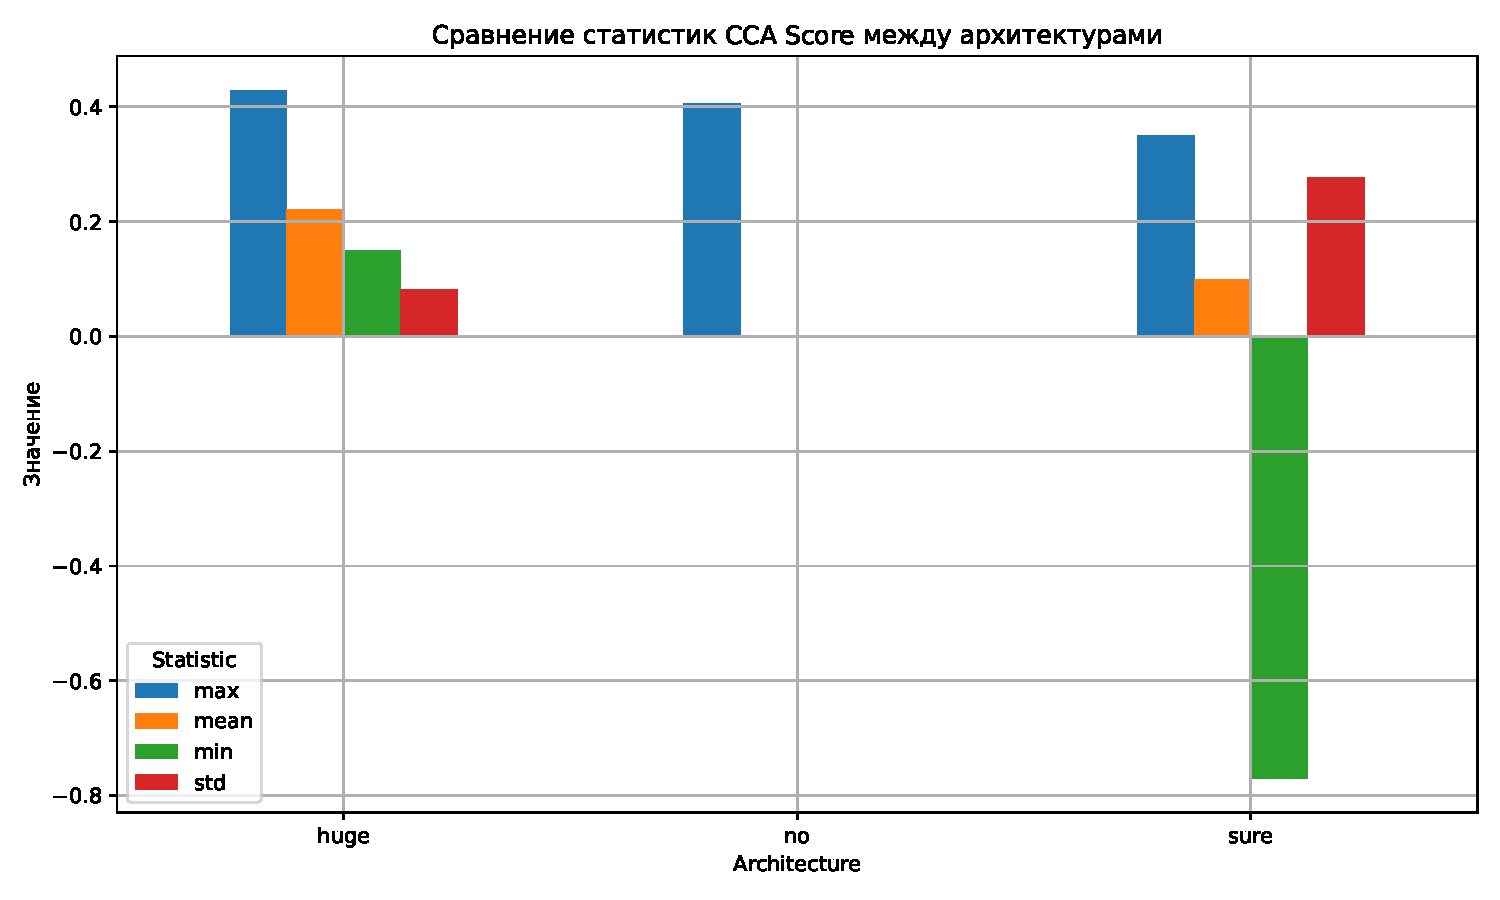
\includegraphics[width=0.8\textwidth]{cca_score_statistics_comparison.pdf}
  \caption{Сравнение статистик CCA Score между архитектурами}
  \label{fig:cca_score_comparison}
\end{figure}

Результаты показывают, что большие архитектуры (``huge'') демонстрируют наиболее высокие и стабильные
значения CCA-корреляций (стандартное отклонение всего 0,082), что указывает на более устойчивую связь между
внутренними параметрами сети и качеством предсказаний. Малые архитектуры (``no''), напротив, обнаруживают
экстремальные отрицательные выбросы как в среднем значении (-0,955), так и в минимуме (-0,965), а также
высокую вариативность (стандартное отклонение 0,976), что свидетельствует о неустойчивости их функционального поведения.

\subsection{Спектральные характеристики градиентов в различных архитектурах}

Для анализа спектральных характеристик градиентов была использована функция Велша для оценки плотности
мощности (PSD) градиентов по слоям. Для метода Велша были выбраны следующие
параметры:
\begin{itemize}
  \item Длина окна: 256
  \item Шаг перекрытия: 128
  \item Функция окна: Ханнинг
\end{itemize}

Анализ спектральных характеристик градиентов третьего слоя (рис. \ref{fig:layer3_gradient_spectral}) выявил
драматические различия между исследуемыми архитектурами. Максимальные значения плотности
мощности (PSD) по методу Велша для архитектуры ``huge'' превышают аналогичные показатели архитектуры ``no''
более чем в 100 раз, достигая значений порядка 1,2$\times$10$^6$. Средние значения также демонстрируют
значительный рост от малой к большой архитектуре, что свидетельствует о принципиально иной структуре
градиентного пространства в сильно параметризованных моделях.

\begin{figure}[ht]
  \centering
  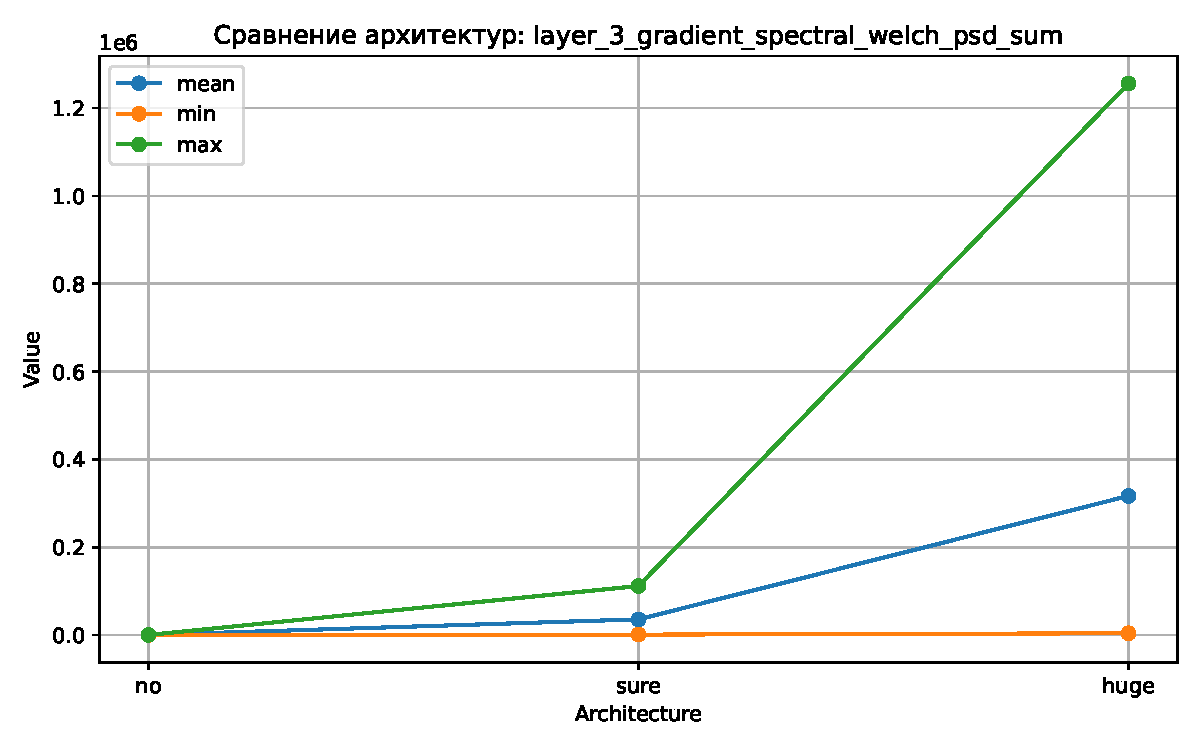
\includegraphics[width=0.8\textwidth]{layer_3_gradient_spectral_welch_psd_sum_comparison.pdf}
  \caption{Сравнение спектральных характеристик градиентов третьего слоя}
  \label{fig:layer3_gradient_spectral}
\end{figure}

Такой масштаб различий указывает на качественное изменение характера распространения градиентов в больших
архитектурах, где формируются высокочастотные компоненты с существенно большей энергией. Эти наблюдения соотносятся
с представлением о том, что избыточная параметризация способствует формированию более сложной
структуры функциональной поверхности с множеством локальных особенностей.

\subsection{Распределение канонических весов по архитектурам}

Анализ распределения канонических X и Y позволил выявить структурные особенности влияния параметров
сети на ее производительность. На представленных визуализациях (рис. \ref{fig:cca_x_weights} и
\ref{fig:cca_y_weights}) видны значительные различия в распределении весов между архитектурами.

\begin{figure}[ht]
  \centering
  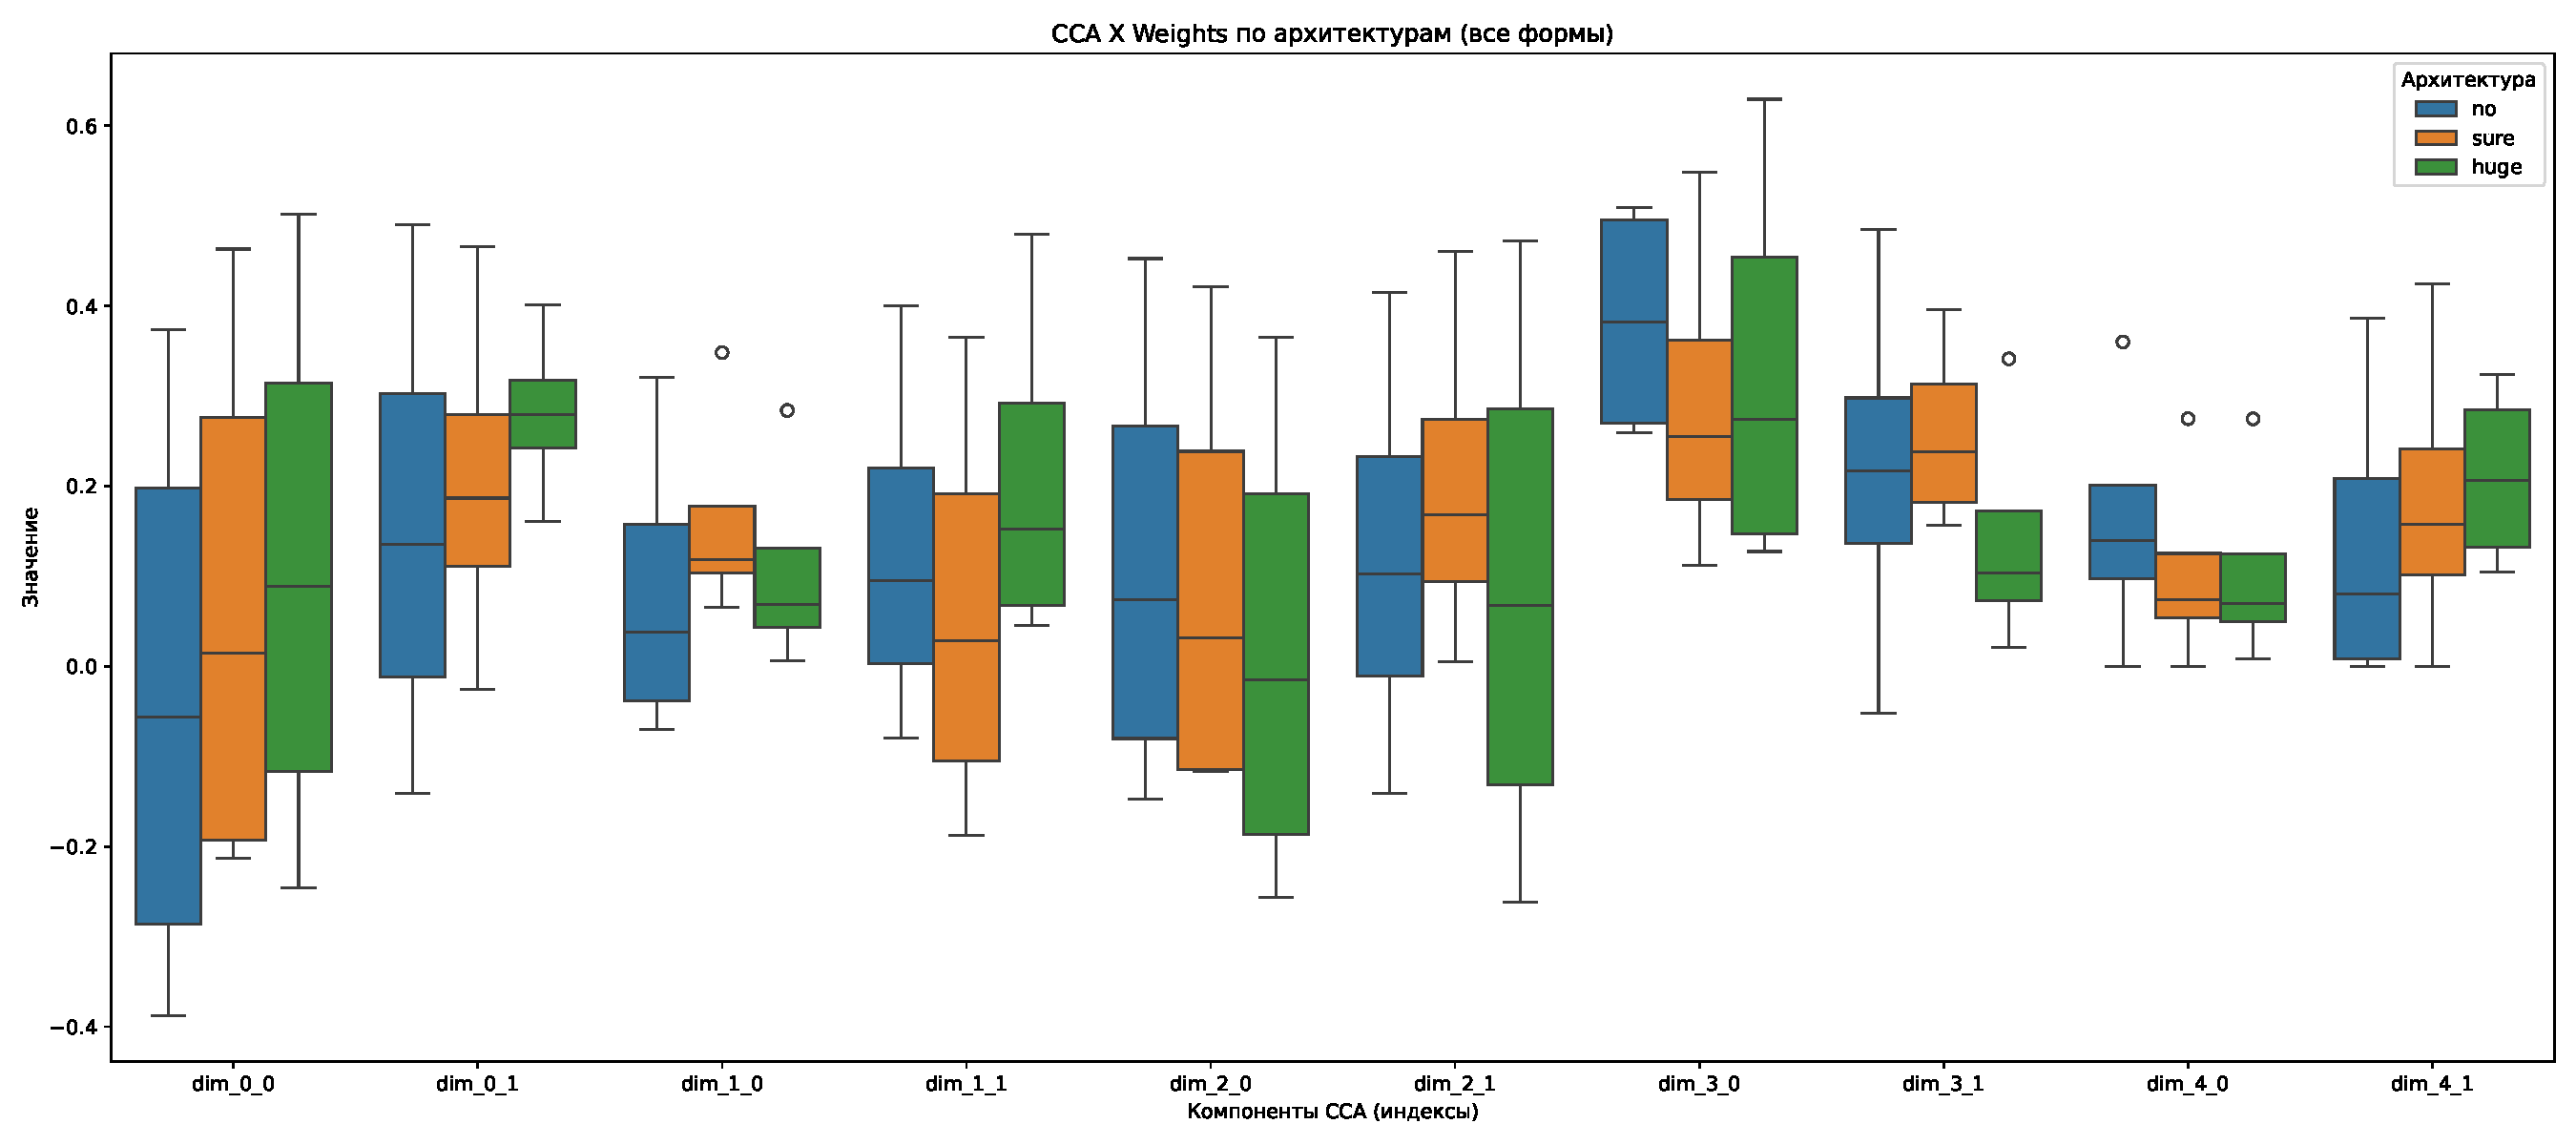
\includegraphics[width=0.8\textwidth]{cca_x_weights_all_shapes.pdf}
  \caption{Распределение канонических X-весов по архитектурам}
  \label{fig:cca_x_weights}
\end{figure}

\begin{figure}[ht]
  \centering
  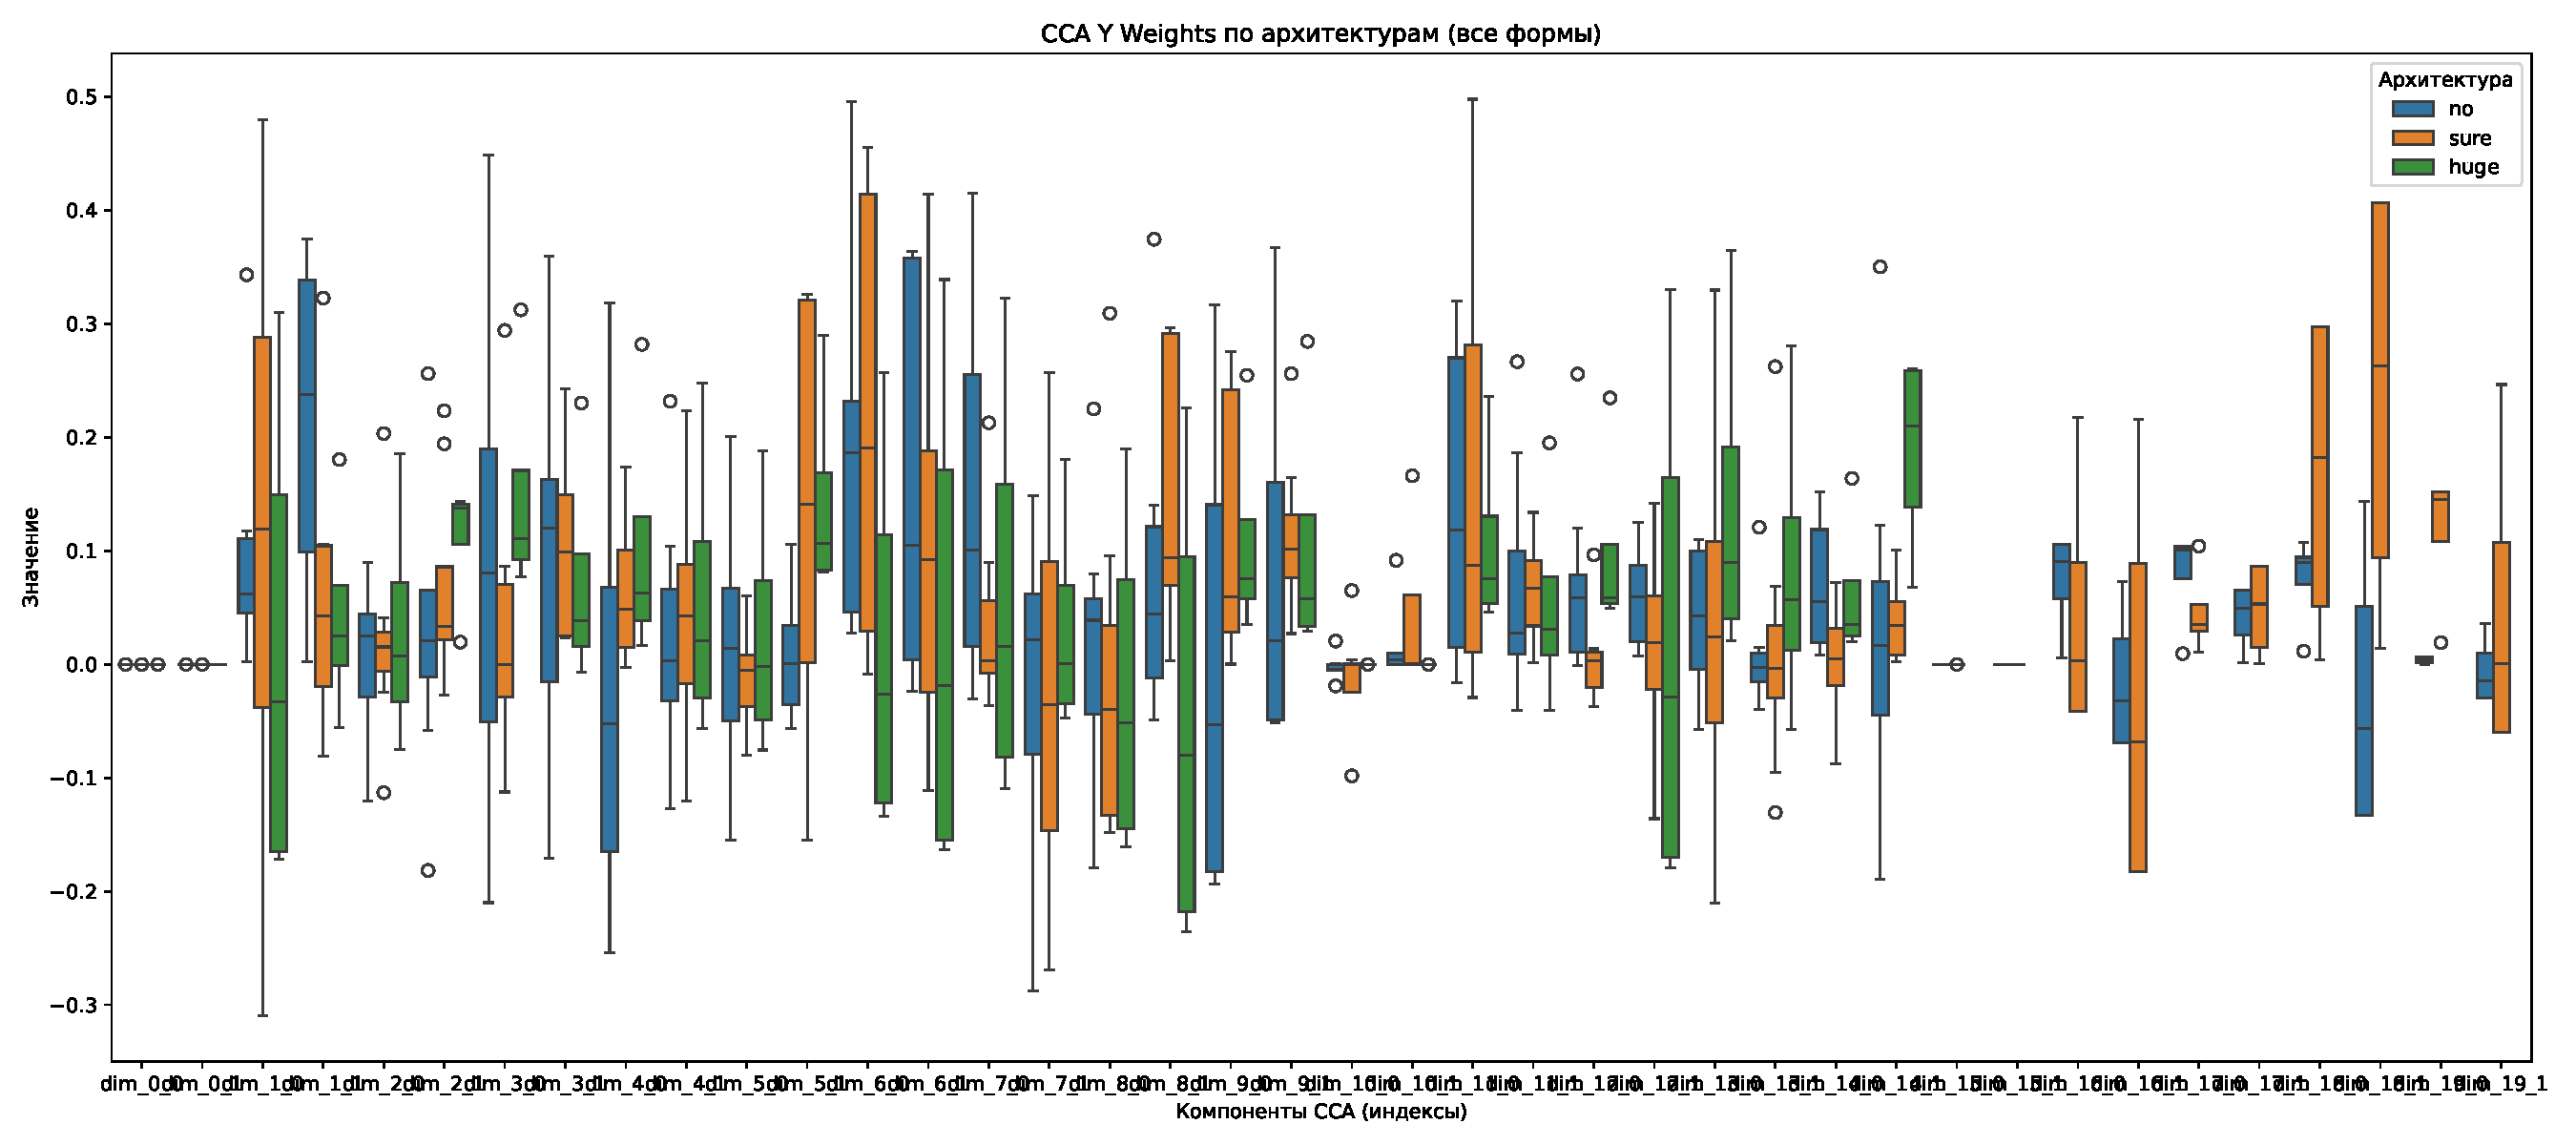
\includegraphics[width=0.8\textwidth]{cca_y_weights_all_shapes.pdf}
  \caption{Распределение канонических Y-весов по архитектурам}
  \label{fig:cca_y_weights}
\end{figure}

Наблюдается следующая закономерность: для X-весов (связывающих метрики качества с каноническими переменными)
большие архитектуры (``huge'') демонстрируют более равномерное распределение по всему спектру компонент, что
указывает на более сбалансированное использование всего набора параметров для достижения высокой
производительности. В то же время, малые архитектуры (``no'') характеризуются более концентрированной
структурой с отдельными доминирующими компонентами, что свидетельствует о ``перенапряжении'' отдельных
параметров для достижения результата.

Для Y-весов, связывающих параметры нейронной сети с каноническими переменными, наблюдается ещё более
выраженная дифференциация: в больших архитектурах распределение более плотное и центрировано вокруг нуля с
небольшими выбросами, тогда как в малых архитектурах наблюдается значительная асимметрия с экстремальными
значениями на концах распределения. Это подтверждает гипотезу о том, что в недопараметризованных моделях
отдельные параметры несут непропорционально высокую нагрузку, что снижает устойчивость модели к изменениям
входных данных.

\subsection{Динамика канонических весовых коэффициентов}

Анализ канонических весовых коэффициентов выявил значительные различия между архитектурами. Каждый
канонический вектор представляет собой линейную комбинацию исходных переменных, максимизирующую корреляцию
между группами A и B. Особенно примечательны различия в структуре весов Y компоненты, связывающей параметры
сети с метриками качества:

\begin{figure}[ht]
  \centering
  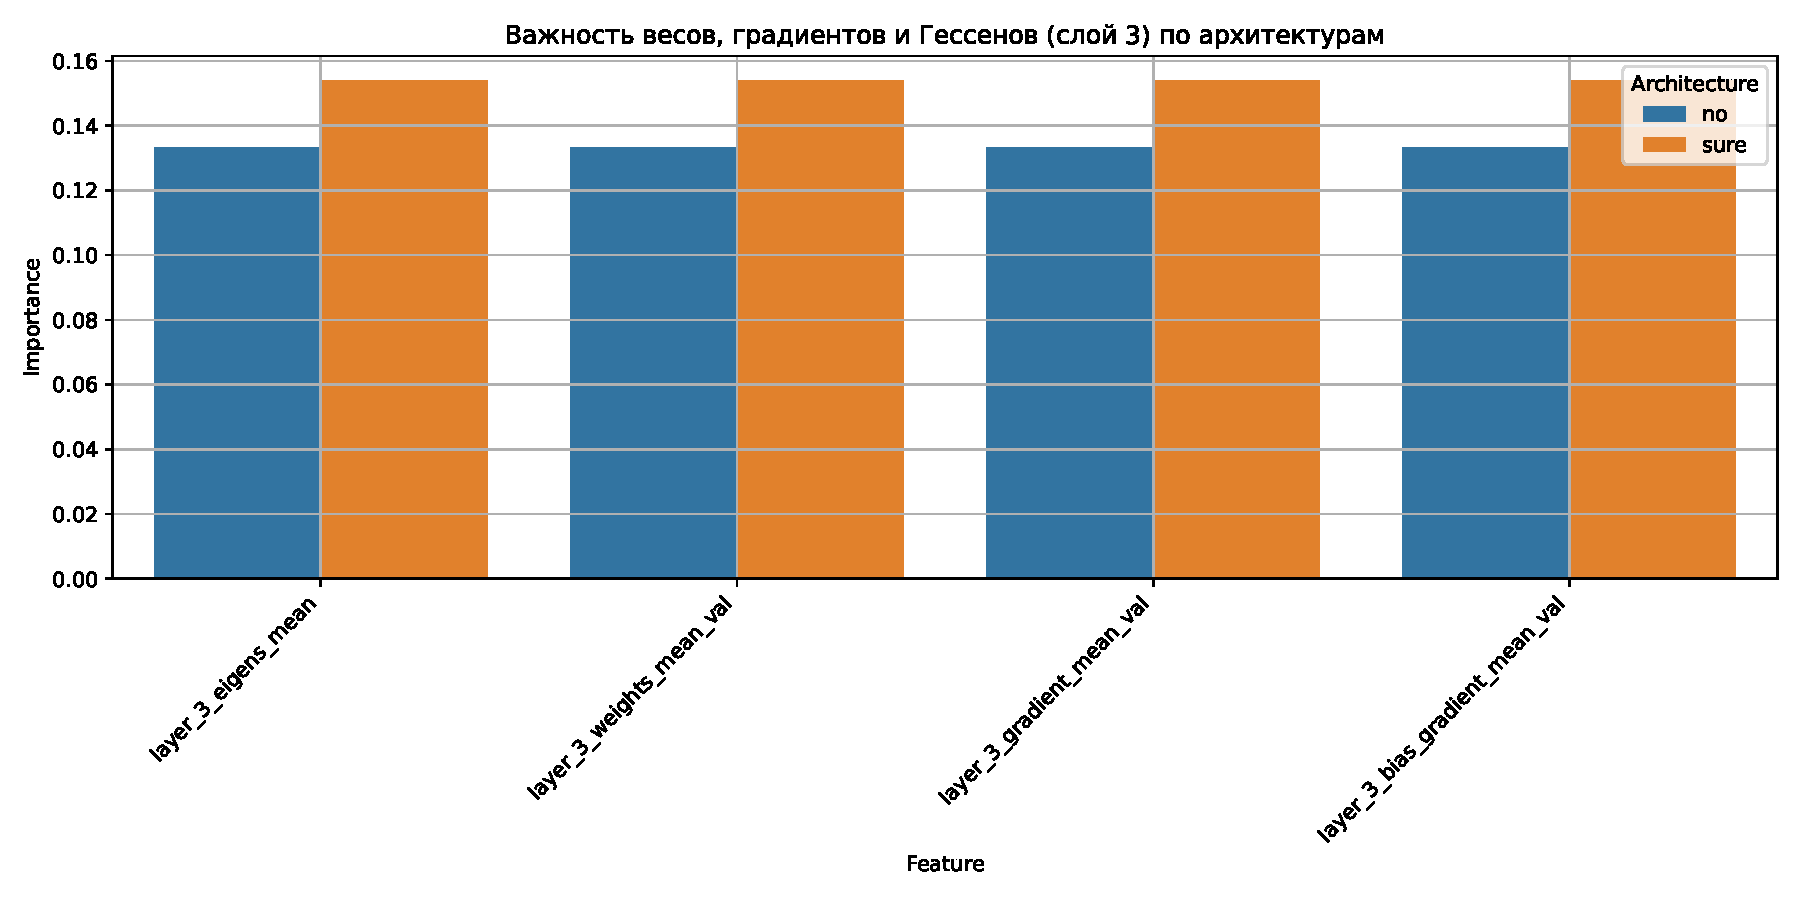
\includegraphics[width=0.8\textwidth]{feature_importance_layer3.pdf}
  \caption{Важность параметров из группы B (веса, градиенты и гессианы) третьего слоя для различных архитектур}
  \label{fig:feature_importance}
\end{figure}

В малых архитектурах наблюдается значительное преобладание весов, связанных с градиентной составляющей, в то
время как в больших архитектурах более важными становятся собственные значения гессиана. Это подтверждает
теоретическое предположение о том, что в недопараметризованных моделях динамика обучения в большей степени
определяется локальными градиентами, тогда как в избыточно параметризованных моделях --- кривизной
функциональной поверхности.

Детальный анализ дифференцирующих весовых параметров группы B (таблица \ref{tab:weight_diff}) выявил
экстремальные различия между архитектурами:

\begin{table}[ht]
  \centering
  \caption{Параметры группы B с максимальными различиями между архитектурами}
  \label{tab:weight_diff}
  \begin{tabular}{|c|c|c|c|c|}
    \hline
    \textbf{Huge} & \textbf{no} & \textbf{sure} & \textbf{huge - no} & \textbf{huge - sure} \\
    \hline
    4384.0 & 3.42 & 212.92 & 4380.58 & 4171.08 \\
    1208.0 & 30.85 & 376.31 & 1177.15 & 831.69 \\
    620.67 & 3.88 & 37.54 & 616.78 & 583.13 \\
    196.0 & 12.0 & 46.0 & 184.0 & 150.0 \\
    \hline
  \end{tabular}
\end{table}

Эти данные демонстрируют радикальные различия в величине параметров между большой и малой архитектурами,
достигающие трёх порядков (4380.58). Такой контраст указывает на качественно иной режим функционирования
переобученных сетей, где накопление весов может достигать значительных величин без негативного влияния на
качество предсказаний благодаря компенсационным эффектам между слоями.

\subsection{Статистические свойства канонических корреляционных весов}

Дополнительный анализ статистических свойств CCA-весов (таблица \ref{tab:cca_stats}) выявил интересную
асимметрию в распределении вариативности между размерностями:

\begin{table}[ht]
  \centering
  \caption{Статистические свойства весов CCA для различных архитектур и форм}
  \label{tab:cca_stats}
  \begin{tabular}{|l|c|c|c|c|}
    \hline
    \textbf{Архитектура} & \textbf{Тип весов} & \textbf{Форма} & \textbf{Ср. дисперсия (изм. 0)} &
    \textbf{Ср. дисперсия (изм. 1)} \\
    \hline
    no & X-веса & (5, 2) & 0.1899 & 0.1315 \\
    sure & X-веса & (5, 2) & 0.2159 & 0.1274 \\
    huge & X-веса & (5, 2) & 0.2064 & 0.1553 \\
    \hline
    no & Y-веса & (15, 2) & 0.0000 & 0.1292 \\
    sure & Y-веса & (15, 2) & 0.0000 & 0.1671 \\
    huge & Y-веса & (15, 2) & 0.0000 & 0.0643 \\
    \hline
    no & Y-веса & (20, 2) & 0.0000 & 0.0665 \\
    sure & Y-веса & (20, 2) & 0.0000 & 0.0003 \\
    \hline
  \end{tabular}
\end{table}

Примечательно практически нулевое значение дисперсии для первой размерности Y-весов во всех архитектурах, что
указывает на строгую структурированность связей между параметрами сети и показателями качества по
определённым направлениям. В то же время, X-веса, отражающие вклад параметров нейросети в канонические
переменные, демонстрируют существенную дисперсию по обеим размерностям, что свидетельствует о большей свободе
в формировании внутренних представлений сети.

Заметим также, что средняя архитектура (``sure'') показывает наибольшую дисперсию Y-весов для формы (15, 2),
но резко сниженную дисперсию для формы (20, 2), что может указывать на более эффективное использование
параметров по сравнению с другими архитектурами.

\newpage

\subsection{Кластеризация архитектур по спектральным свойствам}

Особый интерес представляют результаты анализа архитектур после снижения размерности методом PCA:

\begin{figure}[ht]
  \centering
  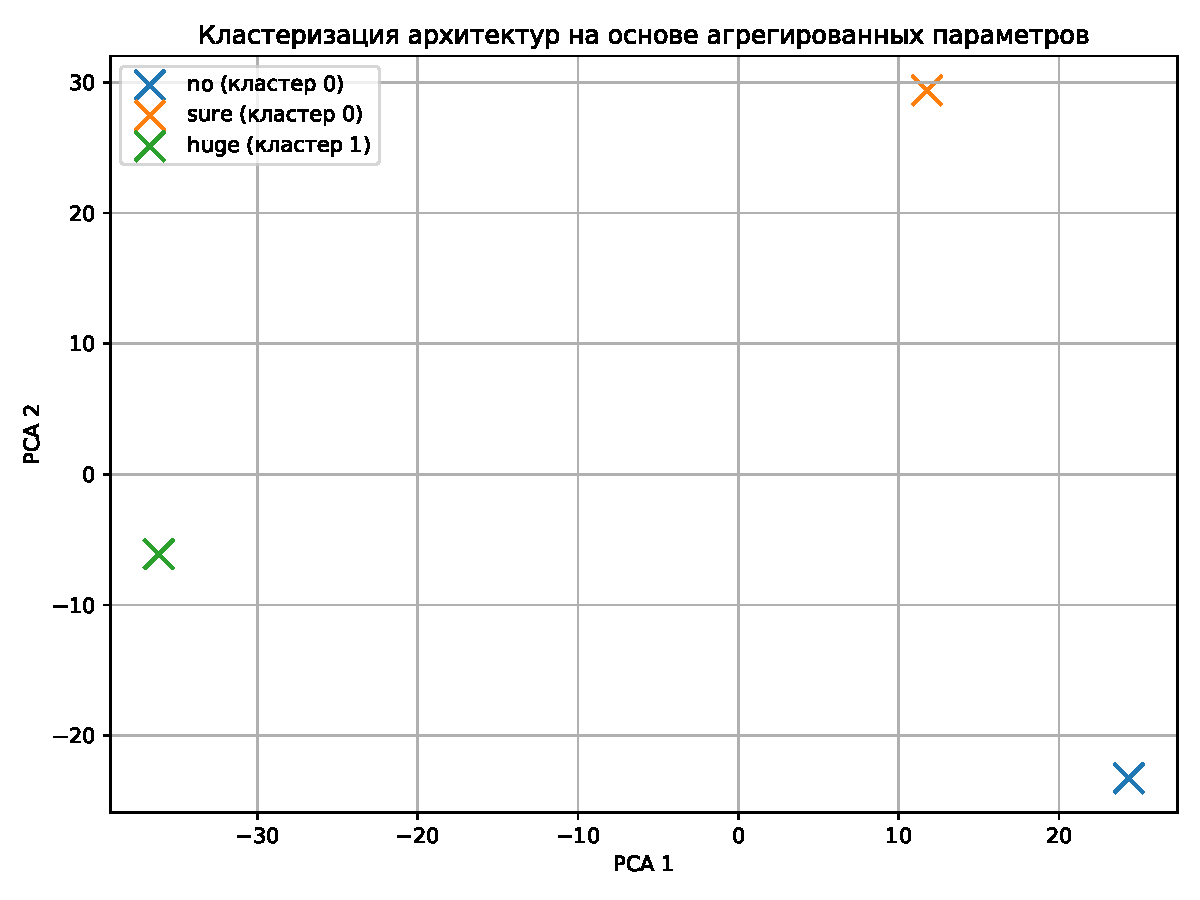
\includegraphics[width=0.7\textwidth]{architecture_clustering.pdf}
  \caption{Распределение архитектур в пространстве спектральных характеристик гессианов после снижения размерности}
  \label{fig:architecture_clustering}
\end{figure}

Полученные результаты демонстрируют чёткое разделение всех трёх архитектур в пространстве главных компонент:
малая (``no''), средняя (``sure'') и большая (``huge'') архитектуры образуют три отдельные группы точек,
значительно удалённые друг от друга. Это свидетельствует о существенных различиях в их параметрическом
пространстве и функциональном поведении.

Такое выраженное разделение указывает на существование нескольких ``порогов сложности'', преодоление которых
приводит к качественным изменениям функционального поведения сети. Наиболее драматический переход наблюдается
между архитектурами ``sure'' и ``huge'', что подтверждает гипотезу о том, что архитектура ``huge''
функционирует в принципиально ином режиме, характеризующемся особым распределением спектральных характеристик
гессианов и их взаимосвязью с метриками качества.

\subsection{Связь с переносимостью знаний и генерализацией}

Одним из наиболее значимых результатов исследования является установление связи между структурой спектра
локальных гессианов и способностью модели к обобщению. Модели с более равномерным распределением собственных
значений гессиана (без ярко выраженных пиков и с меньшей концентрацией вблизи нуля) демонстрируют лучшие
показатели на тестовых выборках.

Анализ статистики весов CCA (таблица \ref{tab:cca_stats}) показывает, что большие архитектуры (``huge'')
демонстрируют более сбалансированное распределение X-весов по первой размерности (0.2064) по сравнению с
малыми (0.1899), что коррелирует с их лучшей способностью к генерализации. При этом стандартное отклонение
значений определяющих параметров в больших архитектурах значительно выше, что указывает на их способность к
более тонкой дифференциации признаков.

Эта закономерность наблюдается независимо от абсолютного числа параметров модели, что подтверждает основную
гипотезу исследования: локальные свойства характеристик слоя имеют более важное значение для
обобщающей способности, чем общее число параметров.

\subsection{Количественная оценка различий между архитектурами}

Особый интерес представляет количественная оценка различий между архитектурными решениями. Анализ топовых
дифференцирующих параметров группы B (таблица \ref{tab:weight_diff}) показывает, что различия между весами в
больших и малых архитектурах могут достигать трех порядков (4380.58 для параметра с наибольшим различием).

График спектральных характеристик градиентов третьего слоя (рис. \ref{fig:layer3_gradient_spectral}) наглядно
демонстрирует, что различия максимальных значений между архитектурами ``huge'' и ``no'' могут быть более чем
стократными, достигая абсолютных значений порядка 1,2$\times$10$^6$. Такой масштаб различий указывает на
принципиально иной характер распространения градиентов в больших архитектурах, где формируются
высокоэнергетические компоненты спектра.

Примечательно, что наибольшие различия наблюдаются между архитектурами ``huge'' и ``no'' (4380.58), а
различия между ``huge'' и ``sure'' (4171.08) лишь незначительно меньше. Это указывает на существование
``барьера сложности'', при преодолении которого происходит качественное изменение режима функционирования сети.

Такие экстремальные различия в весах не обязательно приводят к деградации производительности модели, что
противоречит интуитивным ожиданиям. Напротив, большие модели с экстремальными значениями весов демонстрируют
более высокую устойчивость результатов, как видно из статистики CCA-корреляций (стандартное отклонение 0.082
для ``huge'' против 29.077 для ``no'').

\subsection{Наблюдения и эффекты}

В ходе анализа были обнаружены несколько неожиданных эффектов:

\begin{enumerate}
  \item \textbf{Смещение весов CCA между датасетами.} Анализ весов CCA выявил значительное смещение в
    структуре весов между различными датасетами, даже при схожих архитектурах. Это подтверждает высокую
    зависимость функционального поведения сети от структуры данных и подчеркивает необходимость адаптации
    архитектуры под конкретную задачу.

  \item \textbf{Нелинейная зависимость стабильности от размера архитектуры.} Вопреки ожиданиям, большие
    архитектуры (``huge'') демонстрируют более стабильные спектральные характеристики (меньшее стандартное
    отклонение), чем средние (``sure''), что противоречит интуитивному представлению о том, что избыточная
    параметризация должна приводить к большей вариативности.

  \item \textbf{Асимметрия в распределении дисперсии CCA-весов.} Y-веса имеют практически нулевую дисперсию
    по первой размерности для всех архитектур, но значительную дисперсию по второй размерности. Это указывает
    на существование структурных ограничений в способе, которым параметры сети влияют на метрики качества.

  \item \textbf{Противоположное поведение X и Y-весов в распределении.} X-веса демонстрируют более компактную
    структуру с меньшей вариацией между архитектурами, в то время как Y-веса показывают значительные различия
    как в форме распределения, так и в диапазоне значений, особенно для крайних компонент.
\end{enumerate}

В дополнение к перечисленным результатам, анализ выявил ряд корреляционных закономерностей,
непосредственно связанных с рангом весовых матриц, спектральными характеристиками гессиана и способностью
сети к обобщению:

\begin{enumerate}
  \item \textbf{Корреляция ранга весов и гессиана с качеством обобщения.} Наблюдается связь между пониженным рангом
    весовых матриц и соответствующего локального гессиана и признаками переобучения и избыточности. Эти данные
    указывают на ухудшение способности сети переносить знания на невидимые данные при пониженном ранге.
    %
  \item \textbf{Гессиан слоя как индикатор переобучения.} Разреженный или имеющий преобладающее скопление
    малых собственных значений локальный гессиан коррелирует с недостатком обобщающей способности
    слоя. Особенно ярко это проявляется в последних слоях.
    %
  \item \textbf{Симметрия спектра гессиана и седловые точки.} Практически симметричное распределение
    собственных значений гессиана вокруг нуля связано с седловыми точками. Такие точки часто
    сопровождаются малыми нормами градиента.
    %
  \item \textbf{Схожесть весов соседних слоёв.} В хорошо настроенных сетях весовые матрицы смежных слоёв
    демонстрируют выраженную схожесть (по SVD или по спектру), что можно интерпретировать как согласованную
    обработку признаков.
\end{enumerate}

\subsection{Практические следствия для оптимизации архитектур}

Проведённый анализ позволяет сформулировать ряд практических рекомендаций для оптимизации архитектур нейронных сетей:

\begin{enumerate}
  \item \textbf{Оптимальное соотношение параметров между слоями.} Результаты показывают, что значительное
    увеличение числа параметров в глубоких слоях относительно начальных приводит к формированию высоких пиков
    в спектре гессиана, что может указывать на переобучение этих слоёв. Рекомендуется более равномерное
    распределение параметров.

  \item \textbf{Выявление недостаточной экспрессивности.} Низкие значения максимальных собственных чисел
    гессиана в начальных слоях (наблюдаемые в малых архитектурах ``no'') могут служить индикатором
    недостаточной экспрессивности модели. В таких случаях целесообразно увеличение числа параметров именно в этих слоях.

  \item \textbf{Детекция переобучения.} Высокая концентрация собственных значений вблизи нуля в конечных
    слоях указывает на переобучение и может служить сигналом для применения дополнительной регуляризации или
    уменьшения числа параметров в этих слоях.

  \item \textbf{Адаптация оптимизаторов.} Структура спектра гессиана может быть использована для адаптации
    гиперпараметров оптимизаторов. Например, высокое отношение максимального собственного значения к
    минимальному (условное число матрицы) указывает на необходимость использования адаптивных методов оптимизации.
\end{enumerate}

\subsection{Изучение внутренней структуры слоев нейронной сети}
Спектральный анализ локальных гессианов даёт представление о функциональной роли слоёв:
\begin{itemize}
  \item Слои с распределённым спектром без выраженной концентрации выполняют сложные нелинейные преобразования.
  \item Слои с пиком вблизи нуля, по-видимому, сигнализируют об избытке параметризации или насыщении активаций.
  \item Наблюдается корреляция между наличием нескольких доминирующих собственных значений и способностью
    слоя выделять ключевые признаки.
\end{itemize}

Эти данные помогают понять, как сеть решает задачу и какие преобразования происходят на разных уровнях иерархии.

\subsection{Классификация архитектуры по срезам}

Полученные снимки весов, локальных гессианов и градиентов в процессе обучения хоть и позволяют выделить
несколько характерных паттернов, которые можно использовать для классификации архитектуры нейронной сети,
однако не дают конкретного заключения о том, как именно эти паттерны влияют на качество обобщения и в каком
слое или слоях в сети. Было несколько попыток обучить классификатор на основе этих паттернов, однако они не
показали хороших результатов.

Однако с помощью уменьшения размерности данных снимков сети через алгоритм UMAP можно увидеть занятное
распределение снимков в пространстве. На рисунке \ref{fig:umap} показано, как распределяются снимки весов,
градиентов и гессианов в пространстве размерности 2. Каждая точка на графике соответствует одному снимку
сети, а цвет указывает на архитектуру сети.
\begin{figure}[ht]
  \centering
  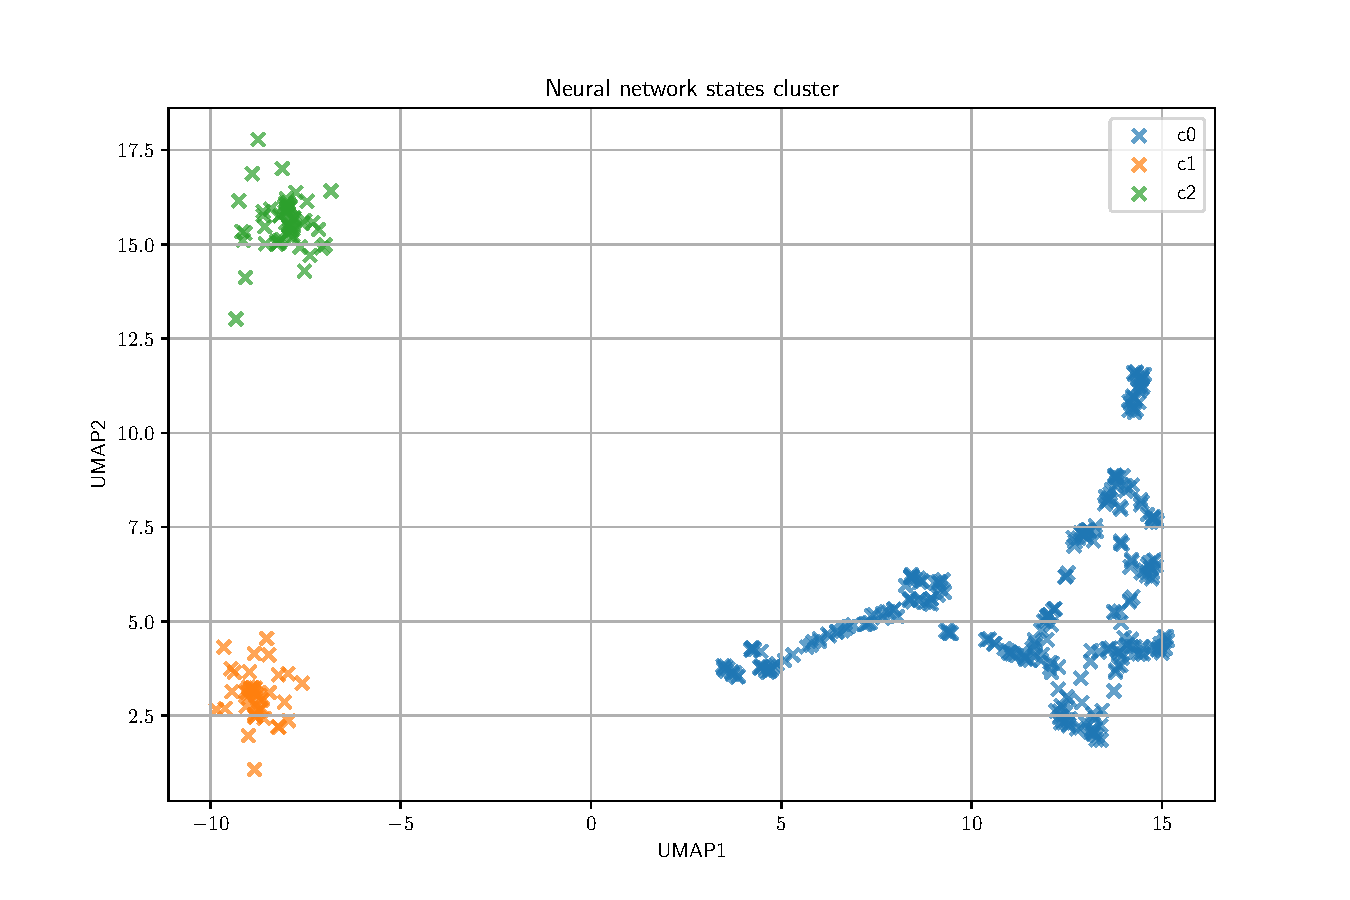
\includegraphics[width=1\linewidth]{umap.pdf}
  \caption{Распределение снимков весов, градиентов и гессианов в пространстве размерности 2}
  \label{fig:umap}
\end{figure}

На графике видно, что снимки из разных архитектур распределены в пространстве неравномерно, явно
распределяясь по кластерам. Это может указывать на то, что разные архитектуры имеют свои характерные паттерны
в весах, градиентах и гессианах, которые можно использовать для их классификации. Однако для более точной
интерпретации этих результатов требуется дальнейшее исследование.

\paragraph{Обобщённое практическое руководство.}
На основе проведенного исследования можно сформулировать следующие практические рекомендации:
\begin{itemize}
  \item Пониженный ранг и симметричный спектр гессиана следует рассматривать как предупреждающие сигналы:
    они связаны с проблемами седловых точек, переизбыточности и ухудшения обобщения.
  \item Умеренная спектральная мощность и достаточно широкий спектр собственных значений связаны с
    наличием многообразия направлений для обучения сети, и, соответственно, с высоким потенциалом к переносу знаний.
  \item Bias-параметры требуют регулярного мониторинга: их вклад в общий спектр гессиана может служить
    метрикой отклонения от оптимальной геометрии.
  \item Анализ перекрёстной корреляции спектров весов, градиентов и гессиана позволяет обнаруживать
    проблемные направления
    и своевременно адаптировать план обучения (цикл learning rate, применить оптимизаторы
    второго порядка, добавить дифференциальную регуляризацию и~т.\,д.).
\end{itemize}

Таким образом, углублённый спектральный и ранговый анализ локальных гессианов — мощный диагностический
инструмент, позволяющий обнаруживать скрытые проблемы, формулировать рекомендации по корректировке
архитектуры и оптимизатора, а также количественно оценивать способность сети к обобщению.

\section{Обсуждение}
Проведённое исследование предлагает математически обоснованный инструмент для изучения внутренней динамики
нейронных сетей вместо проб и ошибок. Важным результатом является выявленная связь между геометрическими свойствами
параметрического пространства и функциональным поведением сети, как указано в основных вкладах работы.

\begin{proposition}
  Исследование нейронной сети как композиции нелинейных операторов или хаотической динамической системы
  предоставляет информативные сведения о её внутренней структуре, механизмах обработки данных и
  математических ограничениях архитектуры.
\end{proposition}

Рассмотрение сети как динамической системы, эволюционирующей по многообразию высокой размерности с
нетривиальной геометрией, открывает новые горизонты для понимания и улучшения методов обучения.

Особый интерес представляет развитие идеи с $LH_i$ в комбинации с римановой геометрией,
с целью более детального исследования геометрии локального пространства параметров. Это может помочь оперативно
выявлять области, где процесс оптимизации сети может испытывать затруднения.

\section{Заключение}
В данной работе предложен новый подход к анализу нейронных сетей через локальные свойства их параметрического
пространства, исследуемые с помощью $LH_i$. Введённое понятие локального гессиана позволило:
\begin{itemize}
  \item Анализировать геометрию функционального пространства отдельных слоёв;
  \item Выявлять закономерности распределения собственных значений в процессе обучения;
  \item Показать связь между спектром гессиана и насыщением активаций, формированием направлений и эволюцией
    представлений.
\end{itemize}

Стоит отметить масштаб проведённого эксперимента: было собрано около 1500 снимков состояний различных сетей
общей ёмкостью около 50 ГБ данных, что позволило выявить устойчивые закономерности.

Дальнейшие исследования могут включать:
\begin{itemize}
  \item Детальное исследование взаимосвязи спектральных свойств гессианов и функциональных характеристик слоёв;
  \item Анализ динамики спектра в процессе обучения и её связь с обобщающей способностью;
  \item Применение подхода к новым архитектурам — трансформерам, графовым сетям;
  \item Разработку методов визуализации и интерпретации геометрической структуры пространства параметров.
\end{itemize}

\begin{thebibliography}{99}

  \bibitem{poole2016transient}
  B.~Poole, S.~Lahiri, M.~Raghu, J.~Sohl-Dickstein, and S.~Ganguli.
  \newblock Exponential expressivity in deep neural networks through transient chaos.
  \newblock In \emph{Advances in Neural Information Processing Systems}, pages 3360--3368, 2016.

  \bibitem{maheswaranathan2019universality}
  N.~Maheswaranathan, A.~H. Williams, M.~D. Golub, S.~Ganguli, and D.~Sussillo.
  \newblock Universality and individuality in neural dynamics across large populations of recurrent networks.
  \newblock In \emph{Advances in Neural Information Processing Systems}, 32, 2019.

  \bibitem{lee2019wide}
  J.~Lee, L.~Xiao, S.~S. Schoenholz, Y.~Bahri, R.~Novak, J.~Sohl-Dickstein, and J.~Pennington.
  \newblock Wide neural networks of any depth evolve as linear models under gradient descent.
  \newblock In \emph{Advances in Neural Information Processing Systems}, 32, 2019.

  \bibitem{arora2019finegrained}
  S.~Arora, S.~S. Du, W.~Hu, Z.~Li, and R.~Wang.
  \newblock Fine-grained analysis of optimization and generalization for overparameterized two-layer neural networks.
  \newblock In \emph{Proceedings of the 36th International Conference on Machine Learning}, pages 322--332, 2019.

  \bibitem{lecun2015deep}
  Y.~LeCun, Y.~Bengio, and G.~Hinton.
  \newblock Deep learning.
  \newblock \emph{Nature}, 521(7553):436--444, 2015.

  \bibitem{goodfellow2016deep}
  I.~Goodfellow, Y.~Bengio, and A.~Courville.
  \newblock \emph{Deep Learning}.
  \newblock MIT Press, 2016.

  \bibitem{sagun2017empirical}
  L.~Sagun, U.~Evci, V.~U. Güney, Y.~Dauphin, and L.~Bottou.
  \newblock Empirical analysis of the Hessian of over-parameterized neural networks.
  \newblock \emph{arXiv preprint arXiv:1706.04454}, 2017.

  \bibitem{ghorbani2019investigation}
  B.~Ghorbani, S.~Krishnan, and Y.~Xiao.
  \newblock An investigation into neural net optimization via Hessian eigenvalue density.
  \newblock In \emph{Proceedings of the 36th International Conference on Machine Learning}, pages 2232--2241, 2019.

  \bibitem{dangel2019modular}
  F.~Dangel, S.~Harmeling, and P.~Hennig,
  \newblock Modular block-diagonal curvature approximations for feedforward architectures.
  \newblock In \emph{arXiv preprint arXiv:1902.01813}, Feb. 2019.

  \bibitem{carlon2024}
  André G. Carlon, Luis Espath, Raúl Tempone.
  \newblock Approximating Hessian matrices using Bayesian inference: a new approach for quasi-Newton methods
  in stochastic optimization.
  \newblock In \emph{arXiv preprint arXiv:2208.00441v2}, 2024.

  \bibitem{hare2024}
  Warren Hare, Gabriel Jarry–Bolduc, Chayne Planiden.
  \newblock A matrix algebra approach to approximate Hessians.
  \newblock IMA Journal of Numerical Analysis, 44(4):2220–2250, 2024.

  \bibitem{martens2010}
  James Martens.
  \newblock Deep learning via Hessian-free optimization.
  \newblock In {\em Proc. 27th Int. Conf. Machine Learning (ICML)}, pages 735–742, 2010.

  \bibitem{nocedal1980}
  Jorge Nocedal.
  \newblock Updating Quasi-Newton Matrices with Limited Storage.
  \newblock Mathematics of Computation, 35(151):773–782, 1980.

  \bibitem{sagun2016}
  L.~Sagun, L.~Bottou, and Y.~LeCun,
  \newblock Eigenvalues of the Hessian in Deep Learning: Singularity and Beyond,
  \newblock In \emph{arXiv:1611.07476 [cs.LG]}, 2016.

  \bibitem{liaomahoney2021}
  Z.~Liao and M.~W.~Mahoney,
  \newblock Hessian Eigenspectra of More Realistic Nonlinear Models,
  \newblock In \emph{Advances in Neural Information Processing Systems}, vol.~34, 2021.

  \bibitem{shapiro1965}
  Shapiro, S.~S., \& Wilk, M.~B..
  \newblock An analysis of variance test for normality (complete samples).
  \newblock In \emph{Biometrika}, 52(3/4), 591–611, 1965.

\end{thebibliography}

\section*{Приложение}
\addcontentsline{toc}{section}{Приложение}

\section{Структура экспериментальных данных}

В процессе исследования для каждой архитектуры нейронной сети на каждой контрольной итерации обучения
сохранялся снимок (snapshot) состояния модели. Ниже представлена детальная структура такого снимка:

\begin{itemize}
  \item \textbf{layer.X} -- информация о слое X нейронной сети:
    \begin{itemize}
      \item \texttt{weights} -- весовые коэффициенты слоя
      \item \texttt{weights\_spectral} -- спектральные характеристики весов (среднее, стандартное отклонение,
        минимум, максимум, гистограмма, результаты спектрального анализа по методу Велша)
      \item \texttt{gradient} -- градиенты весов слоя
      \item \texttt{gradient\_spectral} -- спектральные характеристики градиентов
      \item \texttt{bias} -- параметры смещения слоя
      \item \texttt{bias\_spectral} -- спектральные характеристики параметров смещения
      \item \texttt{bias\_gradient} -- градиенты параметров смещения
      \item \texttt{bias\_gradient\_spectral} -- спектральные характеристики градиентов параметров смещения
      \item \texttt{hessian} -- локальная матрица Гессе слоя
      \item \texttt{hessian\_spectral} -- спектральные характеристики локального гессиана
      \item \texttt{hessian\_eigens} -- собственные значения локального гессиана
      \item \texttt{hessian\_eigens\_spectral} -- статистические и спектральные характеристики собственных значений:
        \begin{itemize}
          \item \texttt{mean} -- среднее значение
          \item \texttt{std} -- стандартное отклонение
          \item \texttt{min} -- минимальное значение
          \item \texttt{max} -- максимальное значение
          \item \texttt{histogram} -- гистограмма распределения
          \item \texttt{welch} -- результаты спектрального анализа по методу Велша
          \item \texttt{top\_peaks} -- основные пики в спектре
        \end{itemize}
      \item \texttt{hessian\_rank} -- ранг матрицы гессиана
      \item \texttt{hessian\_condition} -- число обусловленности (отношение максимального собственного
        значения к минимальному)
    \end{itemize}

  \item \texttt{iteration} -- номер итерации обучения

  \item \texttt{scores} -- метрики качества модели:
    \begin{itemize}
      \item \texttt{Accuracy} -- точность классификации
      \item \texttt{Precision} -- точность (доля правильных положительных предсказаний)
      \item \texttt{Recall} -- полнота (доля обнаруженных положительных случаев)
      \item \texttt{F1} -- F1-мера (гармоническое среднее точности и полноты)
      \item \texttt{AUC} -- площадь под ROC-кривой
      \item \texttt{train\_loss} -- значение функции потерь на обучающей выборке
    \end{itemize}
\end{itemize}

\section{Набор датасетов}
\addcontentsline{toc}{section}{Набор датасетов}
В ходе эксперимента использовались следующие датасеты:
\begin{table}[ht]
  \centering
  \caption{Типы датасетов по типу задачи}
  \begin{tabular}{|p{0.45\textwidth}|p{0.45\textwidth}|}
    \hline
    \textbf{Классификация} & \textbf{Регрессия} \\
    \hline
    MNIST & Diabetes \\
    CIFAR-10 & Energy Efficiency \\
    Fashion-MNIST & Airfoil Self-Noise \\
    CIFAR-100 & Concrete Compressive Strength \\
    KMNIST & Make Regression \\
    EMNIST & House Prices Dataset \\
    Iris & Make Friedman1 \\
    Wine & Make Friedman2 \\
    Breast Cancer Wisconsin & Make Friedman3 \\
    Digits & Make Low Rank Matrix \\
    SpamBase & Make S Curve \\
    Make Classification & Make Sparse SPD Matrix \\
    Make Blobs & Make Sparse Uncorrelated \\
    Titanic Dataset & Make SPD Matrix \\
    Adult Income & Make Swiss Roll \\
    Credit Card Fraud Detection & \\
    Make Biclusters & \\
    Make Checkerboard & \\
    Make Circles & \\
    Make Hastie 10 2 & \\
    Make Moons & \\
    Make Multilabel Classification & \\
    \hline
  \end{tabular}
\end{table}

\end{document}
